\chapter{Theoretical Background}
\label{ch:background}

\section{DMFT}
% TODO explain what x is in our case
% TODO explain trial and result

Dynamical mean-field theory (DMFT)\cite{dmft} is a method to determine the electronic structure of strongly correlated materials. It consists of a self-consistency iteration \(\varphi(x^\ast) = x^\ast\), shown in figure \ref{fig:dmft}, with a very complicated, non-linear function \(\varphi\). $x$ is the self-engery $\Sigma$ and its moments $\Sigma_0$ and $\Sigma_1$.

\begin{figure}[H]
    \centering
    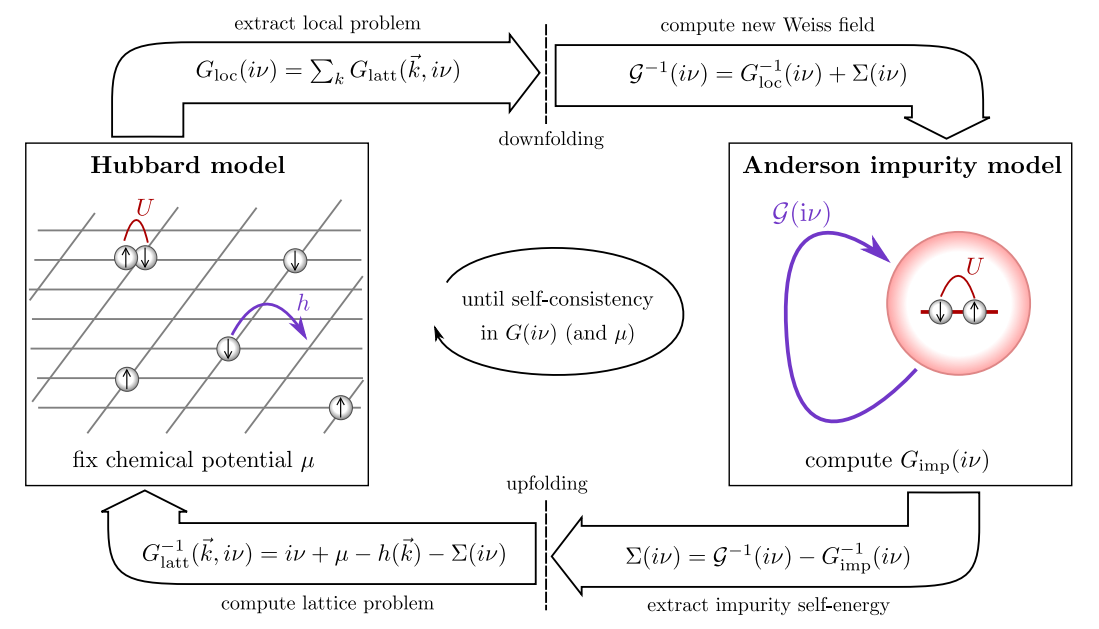
\includegraphics[width=1.0\textwidth]{figures/dmft.png}
    \caption{Self-consistency loop of dynamical mean field theory for a Hubbard-type model. Image taken from Markus Wallerberger's dissertation.\cite{wallerberger2016}}
    \label{fig:dmft}
\end{figure}

\section{Mixing}
Mixing is a technique to improve convergence for self-consistency iteration. The idea is to construct a more effective trial with more information than just the previous result. To be effective such a trial has to be closer to the true value which means we want to extrapolate in terms of iterations.

From now on we will use $x_k$ as the $k$th iteration trial, $\varphi(x_k)$ as the $k$th iteration result and $x^\ast$ as the true value.

The simplest approach is linear mixing
\begin{equation} \label{eq:linmix}
x_{k+1} = (1-\beta) x_k + \beta \varphi(x_k) = x_k + \beta (\varphi(x_k) - x_k)
\end{equation}
with the relaxation parameter \(\beta\).
For \(0 < \beta < 1\) we get an under-relaxation which slows down convergence in some cases, but also dampens oscillations. If the self-consistency iterations diverge, the use of under-relaxation might help.
For \(\beta > 1\) we get over-relaxation which can have predictive behaviour and speed up the convergence but it also amplifies errors and might prevent the convergence of the iteration scheme.

More complex mixing techniques use trials and results of multiple previous iterations and try to combine under-relaxation for robustness and prediction to increase the rate of convergence\cite{anderson_mixing}.

\section{DIIS}
The direct inversion of the iterative subspace (DIIS), also known as Pulay mixing, is an extrapolation technique developed by Peter Pulay\cite{diis_pulay1}\cite{diis_pulay2}. His intention was to accelerate and stabilize the convergence of the Hartree-Fock self-consistent field method. Besides that, DIIS was successfully applied to accelerate the self-consistent field (SCF) approach for density functional theory (DFT) calculations.\cite{diis_restarted}

DIIS uses trials and results of multiple previous iterations, constructs a linear combination of them, and extrapolates a new trial for the next iteration. The coefficients are determined by a least squares optimization.

Pulay's DIIS attempts to construct a better trial by using multiple previous trials and results. The method assumes that a good approximation of the true value \(x^\ast\) can be obtained by a linear combination of the previous trials. That is,
\begin{equation} \label{eq:diis_x}
\overline{x}_{k} = \sum_{j=0}^{m} c_j x_{k-j}
\end{equation}
where \(m\) is the number of previous trials to consider. We can also write this sum in terms of the true value \(x^\ast\) and an error vector \(e_{k} = x^\ast - x_{k}\).
\[\overline{x}_{k} = \sum_{j=0}^{m} c_j (x^\ast + e_{k-j}) = x^\ast \sum_{j=0}^{m} c_j + \sum_{j=0}^{m} c_j e_{k-j}\]
To get close to the true value \(x^\ast\) we set \(\sum_{j=0}^{m} c_j = 1\) and try to minimize the second term \(\sum_{j=0}^{m} c_j e_{k-j}\). But since we do not know the true value \(x^\ast\) we cannot know \(e_{k}\). Therefore, we approximate \(e_{k}\) by the residuals, i.e. \(e_{k} \approx f_{k} = g(x_k) - x_k\):
\[\overline{f}_{k} = \sum_{j=0}^{m} c_j f_{k-j}\].
In order to minimize \(\overline{f}_{k}\) we use the \(l^2\)-norm.

One solution would be to use the Lagrange multiplier technique to satisfy the constraint \(\sum_{j=0}^{m} c_j = 1\) and minimize \(|\overline{f}_{k}|^2\).\cite{diis_math}

However, we can embed the constraint by rewriting \footnotemark
\begin{equation} \label{eq:diis_f}
\overline{f}_{k} = \sum_{j=0}^{m} c_j f_{k-j} = f_k - \sum_{j=1}^{m} \gamma_j {\Delta f}_{k-m+j} = f_k - F_k \Gamma_k
\end{equation}
with \({\Delta f}_{k} = f_k - f_{k-1}\), \(F_k = [{\Delta f}_{k-m+j}]_{j=1..m}\) and \(\Gamma_k = [\gamma_j]_{j=1..m}\).

\footnotetext{For example with \(m=2\) we get \(\overline{f}_{k} = f_k - \gamma_1 {\Delta f}_{k-1} - \gamma_2 {\Delta f}_{k}\ = f_k - \gamma_1 (f_{k-1} - f_{k-2}) - \gamma_2 (f_k - f_{k-1}) = (1-\gamma_2) f_k + (\gamma_2 - \gamma_1) f_{k-1} + \gamma_1 f_{k-2} = c_0 f_k + c_1 f_{k-1} + c_2 f_{k-2}\). Equating coefficients leads to \(\sum_{j=0}^{m} c_j = 1\).}

We minimize \(|\overline{f}_{k}|^2\) by \(\Gamma_k\) and get the solution \footnotemark
\begin{equation} \label{eq:diis_gamma}
\Gamma_k = (F_k^\dagger F_k)^{-1} F_k^\dagger f_k = F_k^+ f_k
\end{equation}

\footnotetext{The last equality is only true if \(F_k^\dagger F_k\) is invertible. The Moore–Penrose inverse exists even if that is not the case.}

Similar to \eqref{eq:linmix} we can construct a new trial with \eqref{eq:diis_x}, \eqref{eq:diis_f} and \eqref{eq:diis_gamma}.
\begin{equation} \label{eq:diis_final}
x_{k+1} = \overline{x}_k + \beta \overline{f}_k = x_k + \beta f_k - (X_k + \beta F_k) (F_k^\dagger F_k)^{-1} F_k^\dagger f_k
\end{equation}

One interpretation of \eqref{eq:diis_final} is that \((F_k^\dagger F_k)^{-1} F_k^\dagger\) is a regression to predict the transformed weights $\Gamma_k$. The regression is trained with \(m\) previous observations and operates on the current observations \(f_k\). $\beta$ decides if we mix trials (\(\beta = 0\)) or results (\(\beta = 1\)).

Variations of the DIIS method exist to further increase the rate of convergence and stability. The restarted Pulay method\cite{diis_restarted} and the periodic Pulay method\cite{diis_periodic} reset the state or use linear mixing in between to reduce side effects of DIIS.

